\documentclass[12pt]{article}
	
%______________________PREAMBULO_________________________

%----------------------Paquetes--------------------------
\usepackage{amsmath,amssymb,amsfonts,latexsym,cancel} % Paquetes de símbolos adicionales.
\usepackage[spanish,es-tabla]{babel} % Idioma español
\usepackage[utf8]{inputenc} % Paquete que nos permite usar los acentos y otros símbolos, directamente del teclado.
\usepackage[T1]{fontenc} % Cambia el tipo de letra
\usepackage{times} % Tipo de letra Times New Roman
\usepackage{graphicx} % Paquete para el manejo de gráficos y figuras en el documento.
\usepackage{geometry} % Permite el manejo de los margenes
\usepackage{fancyhdr} % Permite colocar y manejar el encabezado
\usepackage[breaklinks,colorlinks=true,linkcolor=black,citecolor=blue, urlcolor=blue]{hyperref} % Crea hipervinculo entre secciones y el indice
\usepackage{pstricks}
\usepackage{multicol} % Ayuda a dividir el texto en distintas columnas
%\usepackage{mathpazo} %fuente palatino
%\usepackage{xcolor}
%\usepackage[shortlabels]{enumitem}
%-------------Paquetes para el formato de las citas-------
%\usepackage[hyphens]{url}
%\usepackage{float}
%\usepackage{cite}
%\usepackage{wrapfig}

%-----------------------------ayuda de paquetes--------------------

\spanishdecimal{.}

%------------------------Margenes----------------------------

\newgeometry{bottom = 2.5 cm, top = 2.5 cm, left = 2 cm, right = 2 cm} % Modifica el margen {Abajo, Arriba, Izquierda, Derecha

%----------------------------Interlineado----------------------------------

%\doublespacing
%\onehalfspace
%\singlespace
%\spacing{1.5} % Permite personalisar a gusto
%\setlength{\parskip}{2cm} % Es el espacio entre parrafos

%-----------------------------Sangria---------------------------------------

\setlength{\parindent}{0 cm} % Manipula la sangria

%---------------------Portada------------------

%\title{
%\begin{figure}[h!]
		
%	\centering
%	
\includegraphics[width=\linewidth]{Nom_UAdeC_FCFM.png}  			
			
%\end{figure}
%\huge \textbf{LABORATORIO DE FISICA 3}\\\LARGE TITULO PRACTICA\\}
%\author{ \Large \textbf{Profesor:}\\
%\Large \textbf{Alumno:} Oscar Joel Castro Contreras}
%\date{\today}

%--------------Encabezado y pie de pagina--------------------

\pagestyle{fancy}%Coloca el encabezado en el documento
\lhead[]{Métodos numéricos}%Encabezado izquierda
\rhead[]{Oscar Joel Castro Contreras}%Encabesado derecha
%\chead[]{}%Encabesado central
\renewcommand{\headrulewidth}{0.08 pt}%Coloca linea al pie de pagina

%\lfoot[]{PI}%Pie de pagina izquerdo
%\rfoot[]{PD}%Pie de pagina derecho
\cfoot[]{\thepage}%Pie de pagina central
\renewcommand{\footrulewidth}{0.08 pt}%Coloca linea al pie de pagina

%-----------------------------------------------------------------------------

	\begin{document}
		
		\begin{titlepage}
		
			\centering
			{\bfseries
			\begin{figure}[h!]
				\centering
				
\includegraphics[width=\linewidth]{Nom_UAdeC_FCFM.png} 				
			\end{figure}
			\par}
			\vspace{2cm}
			{\scshape\LARGE Métodos numéricos \par}
			\vspace{3cm}
			{\scshape\Huge \textbf{Método de la Secante} \par}
			\vfill
			{\LARGE \textbf{Profesora:} Maria Guadalupe Godina Cubillo \par}
			\vspace{3cm}
			{\LARGE \textbf{Alumno:} Oscar Joel Castro Contreras \par}
			\vfill
			{\Large \today \par}
			\thispagestyle{empty}
			%\thispagestyle{fancy}
			
		\end{titlepage}
	
		\newpage

		\begin{abstract}
			\noindent En este reporte explico un poco de los métodos que existen para encontrar las raíces de cualquier 
			polinomio o función que tenga raíces, y en específico explico, qué es, en que consiste y cuales son las 
			limitaciones del método de la Secante para encontrar raíces.
		\end{abstract}

		\textbf{Palabras clave:} Raíces, Recta secante, Pendiente, intervalo.

		\section*{\centering Introducción}\label{sec:Introducción}
			Los polinomios son uno de los conceptos más importantes en álgebra y son fundamentales en 
			matemáticas y ciencia en general. Determinar las raíces de un polinomio es uno de los problemas 
			más antiguos en matemáticas.\\
			Puesto que las ecuaciones polinomiales aparecen en un amplio rango de áreas de la ciencia, desde 
			química y física básica hasta economía, el problema de determinar raíces de polinomios es, con 
			frecuencia, un paso obligado en la resolución de problemas.\cite{bib:item1}\\
			La razón principal para resolver ecuaciones no lineales por medio de métodos computacionales es 
			que algunas ecuaciones carecen de solución exacta, excepto por unas pocas. Por lo que existen 
			métodos numéricos diseñados para obtener las raíces, aunque cada uno tiene sus propias 
			limitaciones y defectos. Algunos métodos se muestran en la tabla \ref{tab:1}\cite{bib:item2}\\
			\begin{table}[h!]
				\centering
				\begin{tabular}{|c|c|}
					\hline
					\multicolumn{2}{|c|}{\textbf{Métodos numéricos para obtener raíces}}\\
					\hline
					\textbf{Nombre} & \textbf{Características} \\\hline
					Bisección & Aplicable a funciones no analiticas \\\hline
					Regla falsa & Convergencia lenta en un intervalo grande \\\hline								
					Método de Newton & Rápido, se nesecita calcular derivada \\\hline
					Método de la secante & Rápido, no se requiera calcular derivada \\\hline
				\end{tabular}
				\caption{Métodos numéricos para obtener raíces \cite{bib:item2}}
				\label{tab:1}
			\end{table}\\
			En general, no es posible determinar los ceros de una función, es decir, valores $ x^* $ tal que $f(x^*) = 0 $, 
			en un número finito de pasos. Tenemos que usar métodos de aproximación. Los métodos son 
			usualmente iterativos y tienen la forma: Iniciando con una aproximación inicial $ x_0 $ (o un intervalo $ [a,b] $) , 
			se calculan aproximaciones sucesivas $ x_1,x_2,... $ y elegimos $ x_n $ como aproximación de $ x^* $ cuando se cumpla un 
			criterio de parada dado. A los ceros de un polinomio se les conoce también como raíces.\\
			\textbf{El método de la Secante:}\\
			Un problema potencial en la implementación del método de Newton Raphson es la evaluación de 
			la derivada. Aunque esto no es un inconveniente para los polinomios ni para muchas otras 
			funciones, existen algunas funciones cuyas derivadas en ocasiones resultan muy difíciles de calcular. \cite{bib:item3} \\
			El método de la secante se aproxima utilizando los dos valores $[a,b] $ de iteraciones consecutivas 
			de $ f(x)$. Esto elimina Ia necesidad de evaluar tanto a $ f(x) $ como a $ f'(x) $ en cada iteración. 
			Por lo tanto, el método de la secante es más eficiente, particularmente cuando $ f(x) $ es una 
			función en la que se invierte mucho tiempo al evaluarla. El método de la secante también está 
			íntimamente ligado con el método de la falsa posición. \cite{bib:item2} \\
			Las aproximaciones sucesivas para la raíz en el método de la secante están dadas por un intervalo 
			donde $ [a,b] $, obtenemos la pendiente de la recta formada por el intervalo y por un limite del 
			intervalo y el punto que cruza por el eje x, entonces tenemos que $$ \frac{f(b)-f(a)}{b-a} = \frac{0-f(a)}{x-a} $$ 
			y llegamos a que la raíz es $$ x = a - \frac{f(a)(b-a)}{f(b)-f(a)} $$ que es parecida a la de Newton Raphson.
			

		\section*{\centering Metodología}\label{sec:Metodologia}
			El método de la Secante es parecido al de Newton Raphson, este parte de un intervalo $ [a,b] $, al 
			evaluar la función $ f(x) $ en el intervalo obtenemos 2 puntos $ (a,f(a)) $ y $ (b,f(b)) $. Por estos 
			puntos se traza una recta secante que cruce por los 2 puntos. Después a partir de la fórmula de la 
			recta, obtenemos la pendiente, con la ayuda de los puntos encontrados al evaluar el intervalo y 
			tenemos que la pendiente es $$ m_1 = \frac{f(b)-f(a)}{b-a} $$, después volvemos a calcular la 
			pendiente pero con el punto por el que la recta cruza el eje $ x $, y uno de los puntos obtenidos, 
			entonces tenemos los puntos $ (a,f(a)) $ y $ (x,0) $, calculamos la pendiente $$ m_2 = \frac{f(a)-0}{x-a} $$, 
			igualamos esta pendiente y despejamos para $ x $ $$ m_1 = m_2 $$ $$ \frac{f(b)-f(a)}{b-a} = = \frac{f(a)-0}{x-a} $$ 
			llegamos a que la aproximación de la raíz es $$ x = a - \frac{f(a)(b-a)}{f(b)-f(a)} $$, ahora evaluamos la 
			aproximación en la función $ f(x) = 0 $ si es igual a cero se encontró la raíz si no, esté valor obtenido, 
			lo cambiamos por un límite del intervalo inicial, y volvemos a iterar con el nuevo punto, hasta que llegamos a la raíz. 
			Este método es como una combinación de Newton Raphson y Regla falsa.\\
			El criterio para parar las iteraciones es el mismo que bisección, ragla falsa y Newton Raphson, está dado por el número de cifras 
			significativas que queramos, de aquí obtenemos una tolerancia, la cual en cada interacción se 
			compara con el error relativo y absoluto, si uno de los errores es menor o igual a la tolerancia, 
			detener las interacciones.\\
			La parte mas importante del programa es el calculo de la aproximacion de la raiz
			\begin{center}
				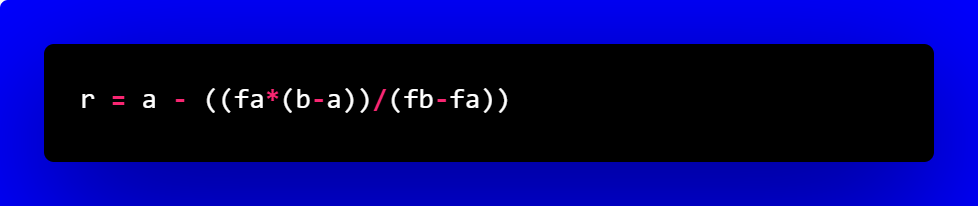
\includegraphics[width=\linewidth]{Figura 1.png}
				Figura 1: Formula de aproximacion a la raiz por el metodo de la Secante		
			\end{center}

		
		\section*{\centering Resultado}\label{sec:Resultado}
			Si tomamos el polinomio $ x^3-2x^2-1 $ y damos de intervalo inicial $ [1,3] $. Hacemos 
			la evaluación para obtener la raíz con 5 cifras significativas, el programa nos arroja
			\begin{multicols}{2}
				\begin{center}
					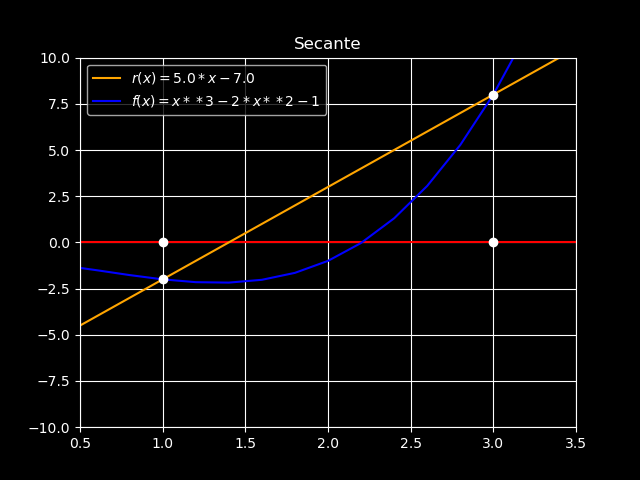
\includegraphics[width=\linewidth]{Grafica 1.png}
					Grafica 1: Recta Secante que cruza $ x^3-2x^2-1 $ \columnbreak en el intervalo donde $ x = [1,3] $.\\
					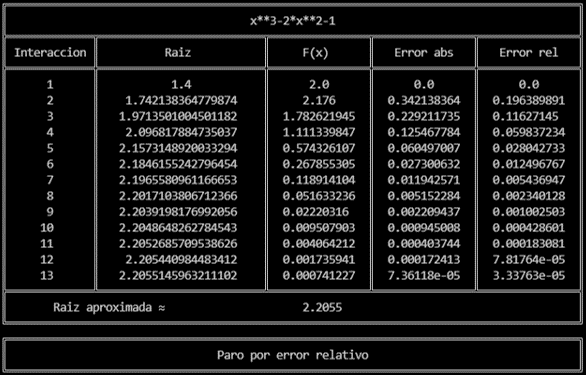
\includegraphics[width=\linewidth]{Tabla 1.png}
					Tabla 2: Iteraciones a la aproximación de la raíz de la función $ x^3-2x^2-1 $.
				\end{center}
			\end{multicols}
			Observamos que la aproximación a la raíz es $ 2.2055 $, con 13 iteraciones. El criterio de paro fue 
			por el error relativo.
		\section*{\centering Observación}\label{sec:Observacion}
			El método tiene algunas limitaciones, casi las mismas que el método de Newton Raphson en 
			algunos casos la diferencia de $ f(b) - f(a) $ es igual a cero ya $ f(a) $ es igual que $ f(b) $, cuando ocurre 
			esto la recta secante no cruzar por el eje $ x $, por lo que en estos casos el método se parar y se le 
			pedir al usuario que coloque un intervalo inicial diferente. Otra de las limitaciones es cuando 
			la función no tiene raíces reales o cuando se coloca un intervalo inicial muy lejano a la raíz, 
			en estos casos el método nunca deja de iterar, por lo que se le debe de dar un paro a una cierta cantidad 
			de iteraciones, el máximo de iteraciones que le coloque a mi programa es de 1000.
		\section*{\centering Conclusión}\label{sec:Conclusion}
			En conclusión, el método de la Secante toma un intervalo inicial $ [a,b] $ con el que se hace un 
			recta secante que cruza por el eje $ x $, y con la formula obtenida de la pendiente de la recta 
			secante, se va internado hasta llegar a un buena aproximación de la raíz. Las limitaciones del 
			método son cuando se tiene un intervalo que al evaluar en la función se tiene que $ f(a) $ y $ f(b) $ 
			son iguales, en este caso la recta no cruza el eje $ x $ y cuando no tiene raíces reales o cuando se 
			coloca un intervalo inicial muy lejano a la raíz el método nunca se detiene.

		\centering
		\begin{thebibliography}{10}
			\bibitem{bib:item1} de la Vega, H. M. El calculo de raıces de polinomios. Una historia sin fin. Recuperado de
							\href{http://www.matedu.cinvestav.mx/~elcalculoysuensenanza/investigacion/articulosPDF/Madrid.pdf}{Pagina web de \cite{bib:item1}}.
			\bibitem{bib:item2} Nakamura, S. (1998). Metodos Numericos Aplicados Con Software. En Solución de ecuaciones no lineales (Primera ed., pp. 62–63). Prentice Hall.
			\bibitem{bib:item3} Mora, W. (2010). Introducción a los Métodos Numéricos. Implementaciones en R. Ecuaciones no lineales (Primera ed., pp. 95,110) Recuperado de
							\href{https://tecdigital.tec.ac.cr/revistamatematica/Libros/WMora_MetodosNumericos/2017_Principal_MetodosNumericos-con-R.pdf}{Pagina web de \cite{bib:item3}}. 
							\bibitem{bib:item4} Chapra, S. (2015). Métodos numéricos para ingenieros. RAICES DE ECUACIONES (7.a ed., pp. 91–180). Editorial McGraw-Hill.				
			
		\end{thebibliography}

	\end{document}